\documentclass{article}
\usepackage{graphicx} % Required for inserting images
\usepackage{geometry}
\usepackage{circuitikz}
\usepackage{siunitx}
\usepackage{CJKutf8}
\usepackage{amsmath}
\usepackage{amssymb}
\usepackage{caption}
\usepackage{float}
\usepackage{subcaption}
\geometry{top=5mm, left=30mm, a4paper}

\title{Diode Circuits Report}
\author{梁程捷 (B11901136), 吳奕娃 (B11901080)}
\date{}


\begin{document}
\begin{CJK*}{UTF8}{bkai}

\maketitle
%===========Diode Circuit================
\section{Diode Circuits}
\textbf{cut-in-voltage $v_D$ = 0.6 V}
\begin{figure}[h]
    \begin{center}
    
        \begin{subfigure}[b]{0.35\textwidth}
            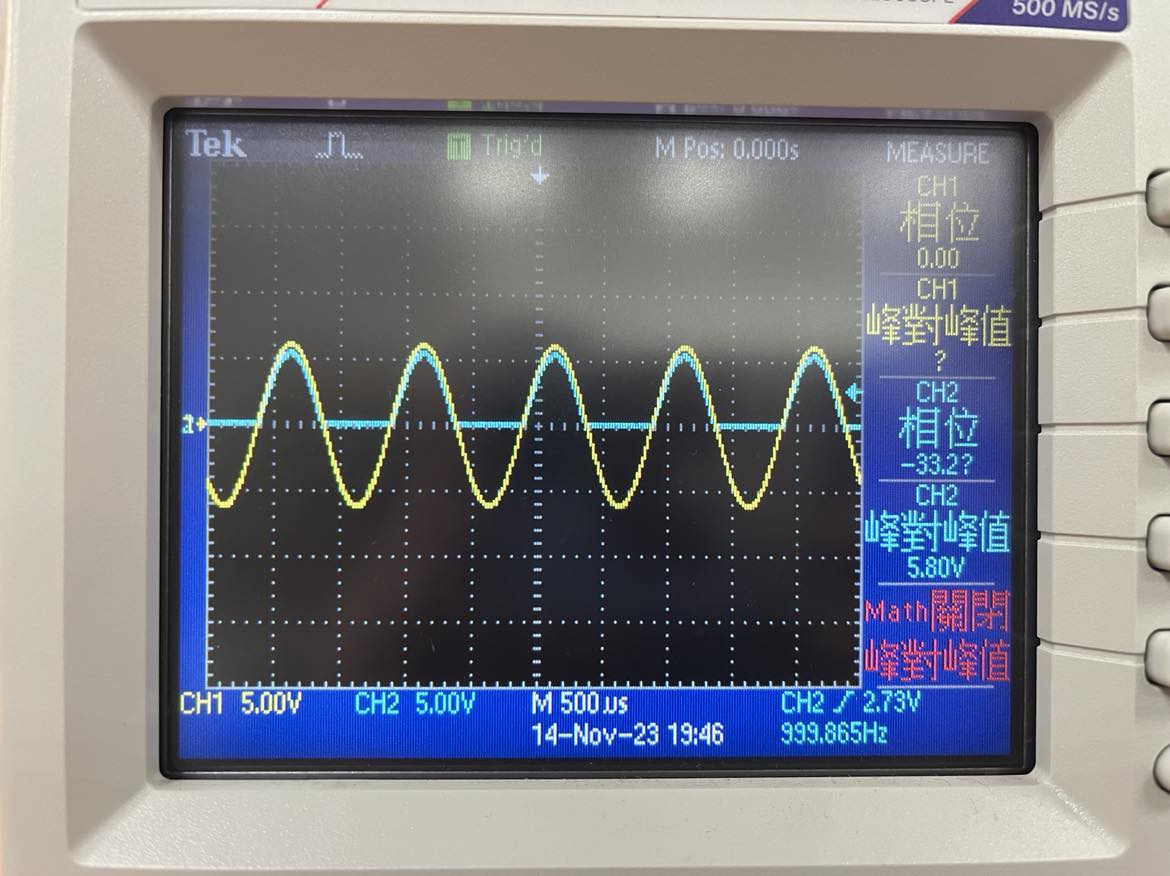
\includegraphics[width=\textwidth]{diode_yt.jpg}
            \caption{Diode: Y-t mode}
        \end{subfigure}
        ~
        \begin{subfigure}[b]{0.35\textwidth}
            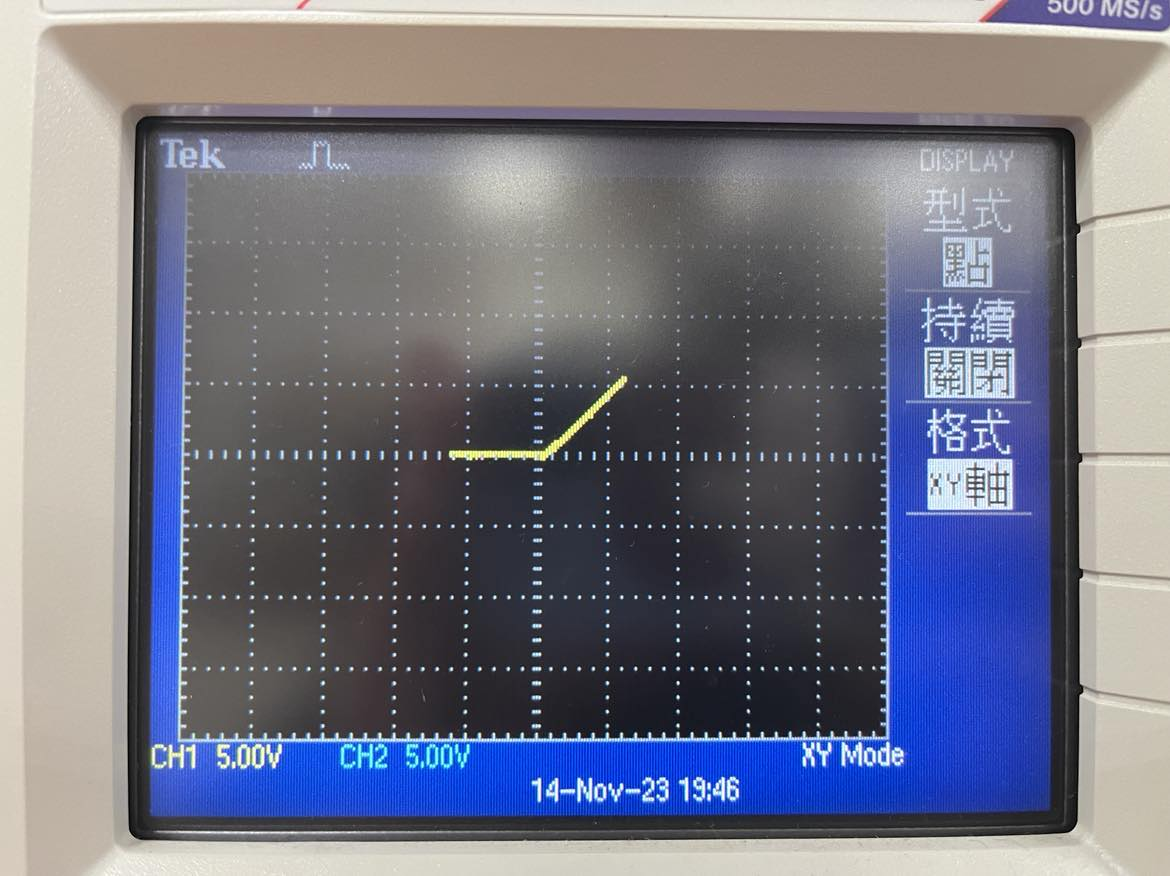
\includegraphics[width=\textwidth]{diode_1k.jpg}
            \caption{Diode: X-Y mode, $f$= 1 k\unit{\hertz}}
        \end{subfigure}
        
        \begin{subfigure}[b]{0.3\textwidth}
            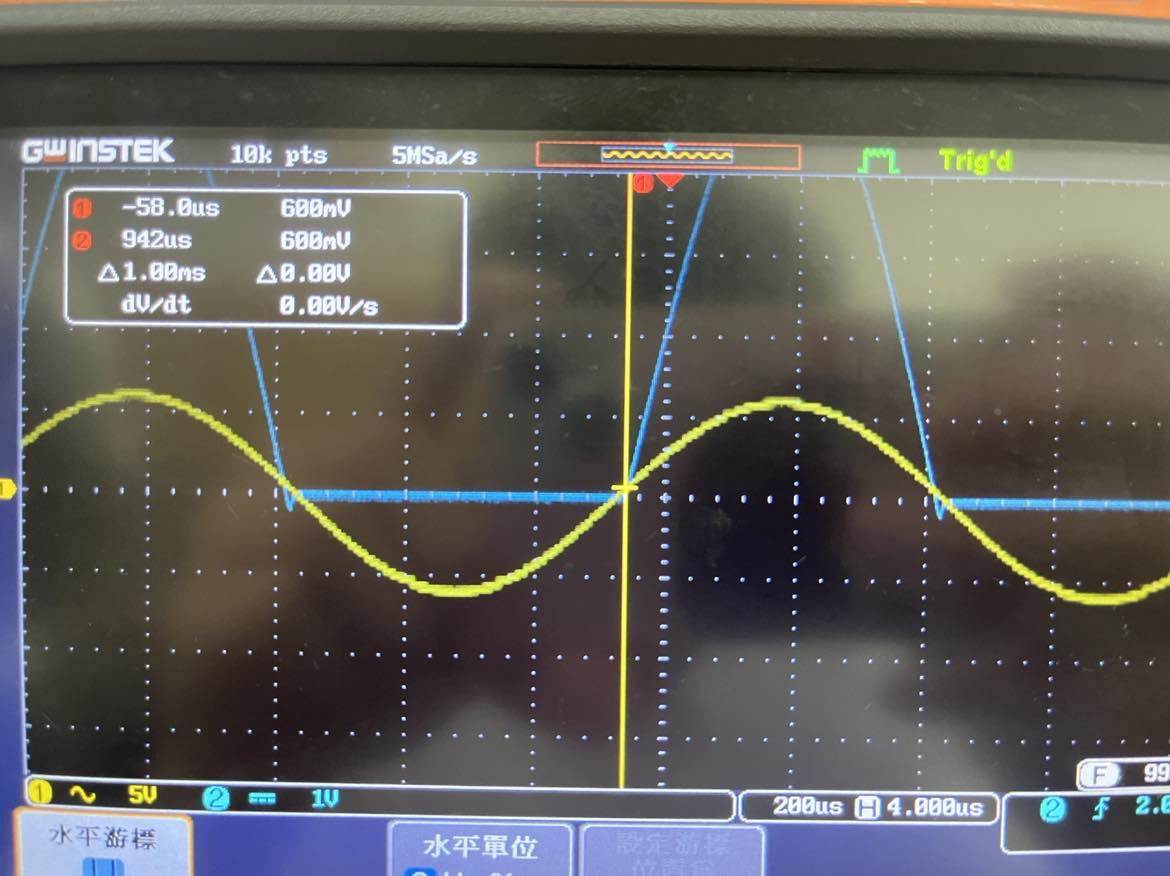
\includegraphics[width=\textwidth]{cut_in_voltage.jpg}
            \caption{Diode: cut-in voltage \\measurement}
        \end{subfigure}
        ~
        \begin{subfigure}[b]{0.3\textwidth}
            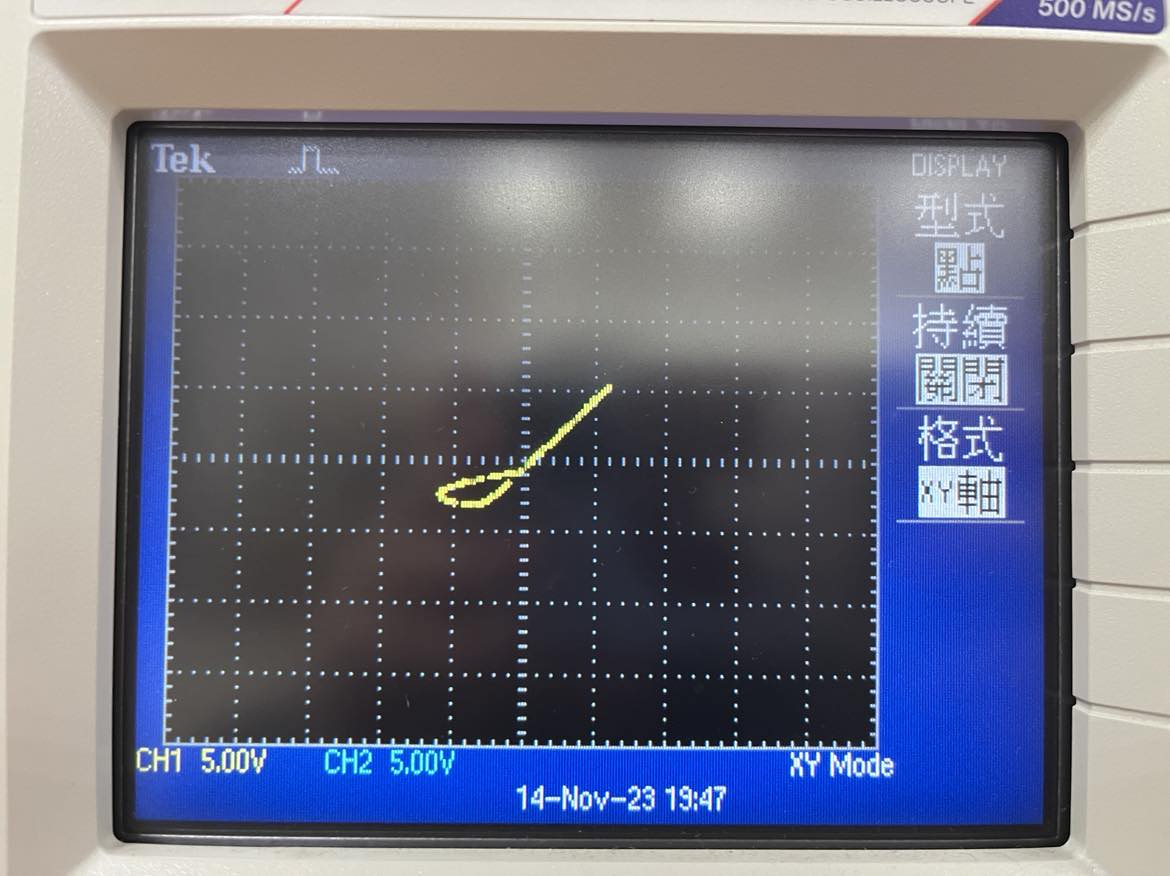
\includegraphics[width=\textwidth]{diode_200k.jpg}
            \caption{Diode: X-Y mode,\\ $f$= 200 k\unit{\hertz}}
        \end{subfigure}
        ~
        \begin{subfigure}[b]{0.3\textwidth}
            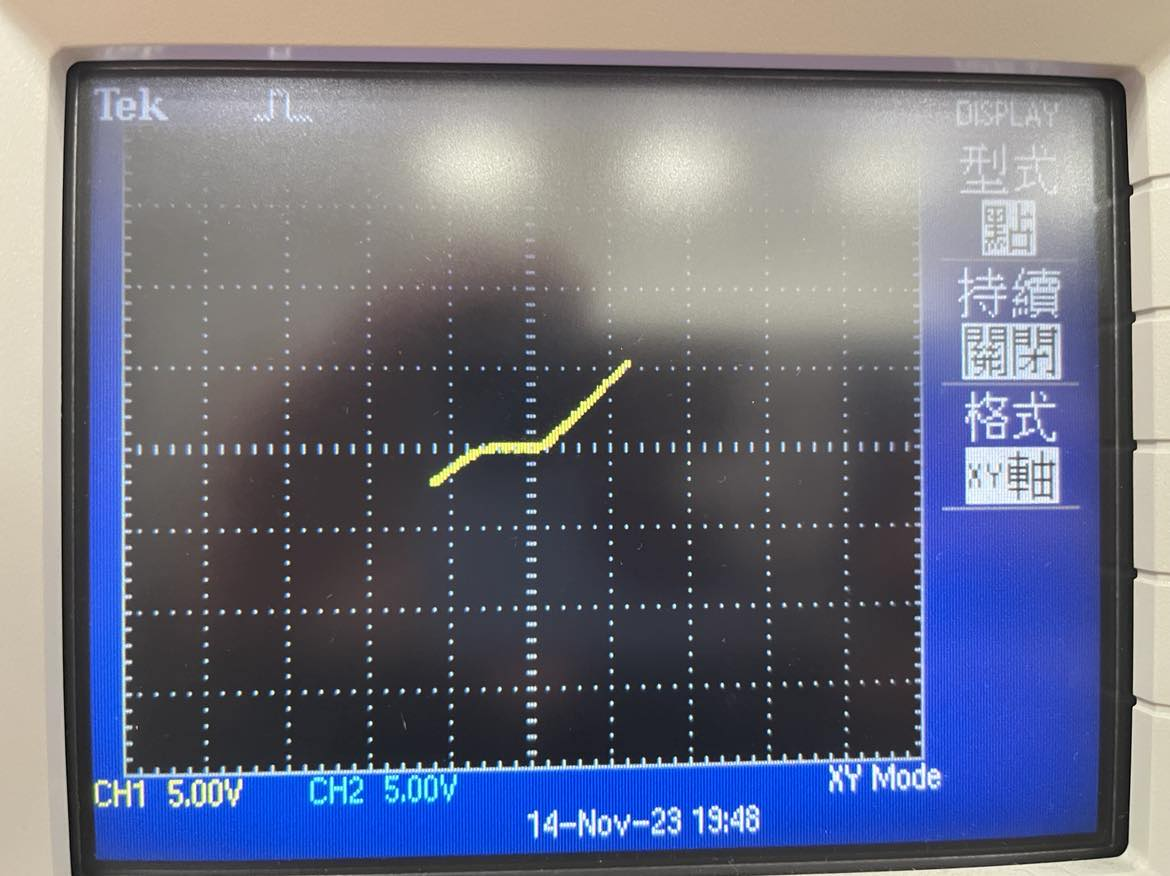
\includegraphics[width=\textwidth]{zener_xy.jpg}
            \caption{Zener diode $i-v$ curve}
        \end{subfigure}
    \end{center}   
    \end{figure}

%===========Voltage regulator================
\section{Voltage regulator}
\begin{table}[H]
    \begin{center}
    \begin{tabular}{|c|c|c|c|c|}
        \hline
        $VR$ (\unit{\kilo\ohm}) & $V_o$ & $I_1$ (\unit{\milli\ampere}) & $I_Z$ (\unit{\milli\ampere}) &  $I_2$ (\unit{\milli\ampere})\\
        \hline\hline
        2	 & 1.507 & 0.754 & 0.001 & 0.754 \\
        20   & 3.941 & 0.510 & 0.304 & 0.204 \\
        400	 & 4.096 & 0.494 & 0.485 & 0.010 \\
        600	 & 4.098 & 0.494 & 0.487 & 0.007 \\
        800	 & 4.098 & 0.494 & 0.489 & 0.006 \\
        1000 & 4.098 & 0.494 & 0.475 & 0.002 \\
     \hline
    \end{tabular}
    \caption{voltage regulator raw experimental data}
    \end{center}
\end{table}
\textbf{Conclusion: output voltage $V_o$ is very stable with large load resistance.}
\end{CJK*}
\end{document}